%!TEX root = ../thesis_a4.tex

\chapter{Applications in Musicology}
\label{sec:musicology}

\section{Introduction}
\label{sec:musicology:introduction}

\section{Building Culture-specific Knowledge Bases: The Flamenco Case}

\subsection{Introduction}\label{sec:introduction}

Music context information is now playing a key role in MIR research. Multimodal approaches, semantic approaches, and text-IR approaches have shown important achievements in typical MIR problems, such as music recommendation and discovery, genre classification, or music similarity \cite{Schedl2014}. Therefore, collecting and storing music context information may be extremely useful for the MIR research community \cite{Oramas2014}. There are some broad repositories of music context information such as MusicBrainz\footnote{http://musicbrainz.org} or Discogs\footnote{http://www.discogs.com/}. Although some of these repositories are very complete and accurate, there is still a vast amount of music information out there, which is generally scattered among different sources on the Web. Hence, harvesting and combining that information is a crucial step in the creation of practical and meaningful music knowledge bases. In addition, the creation of genre-specific knowledge bases may be very valuable for research and dissemination purposes, and particularly to non-western music traditions. 
%However, to the best of our knowledege, not many initiatives have been focused on this direction.

In this paper, we propose a methodology for the creation of a genre-specific knowledge base; in particular, a knowledge base of flamenco music. The proposed methodology combines content curation and knowledge extraction processes. First, an important amount of information is gathered from different data sources, which are subsequently combined by applying pair-wise entity resolution. Next, new knowledge is extracted from unstructured harvested texts and employed to populate the knowledge base. For this purpose, an entity linking system has been expressly developed. Finally, the content of the knowledge base is used to compute artist relevance and results are evaluated according to flamenco experts criteria. The content of the knowledge base is freely available and downloadable as data dumps in RDF and JSON formats.

The remainder of the paper is organized as follows. In Section~\ref{sec:flamenco}, an introduction to flamenco music is presented. In Section~\ref{sec:related_work}  some relevant prior work is briefly surveyed. Section~\ref{sec:flabase} describes the structure of the knowledge base. Next, in Section~\ref{sec:kb_curation} the process of content curation is explained. Section~\ref{sec:kb_extraction} shows the methodology applied for knowledge extraction. In Section~\ref{sec:statistics} artist relevance is computed and some statistics about the content are laid out. Finally, Section~\ref{sec:conclusion} concludes the paper and points out for future lines of work.


\subsection{Flamenco music}\label{sec:flamenco}


%Flamenco is music characterized by two apparently contradictory yet complementary elements. On the one hand, improvisation and spontaneity, all spurred on by both the performers and the audience. On the other hand, flamenco music leans on an extremely stable organization of the musical material, without which the improvisation could not take place. 
Several musical traditions contributed to the genesis of flamenco music as we know it today. Among them, the influences of the Jews, Arabs, and Spanish folk music are recognizable, but indubitably  the imprint of  Andalusian Gypsies' culture is deeply ingrained in flamenco music. 
Flamenco occurs in a wide range of settings, including festive \textit{juergas} (private parties), \textit{tablaos} (flamenco venues), concerts, and big productions in theaters. In all these settings we find the main components of flamenco music: \textit{cante} or singing, \textit{toque} or guitar playing, and \textit{baile} or dance. According to Gamboa~\cite{gamboa-05}, flamenco music grew out of the singing tradition, as a melting process of all the traditions mentioned above, and therefore the role of the singer soon became dominant and fundamental. \textit{Toque}  is subordinated to \textit{cante}, especially in more traditional settings, whereas \textit{baile} enjoys more independence from voice. 

%A \textit{cante}, in its most traditional presentation (voice and guitar), is composed of a small set of pieces sung in a more or less fixed order, similar to sections in classical or popular music. The dialogue between the voice and the guitar as well as the guitar playing itself are distinctive features of each \textit{cante}. Each \textit{cante} is made up of a set of verses (\textit{coplas} or \textit{tercios}).  The guitarist usually plays an introduction where tonality, rhythm, meter, and tempo of the \textit{cante} are set.

%Harmonically, flamenco \textemdash at least the more traditional one\textemdash~use three modes mainly: major mode, minor mode, and Phrygian mode with a major third degree. A very common chord progression in flamenco is the Andalusian cadence. In E, this cadence corresponds to Am-G-F-E, which can be seen in modal and tonal contexts. Melodically, several features are characteristic of flamenco music: short tessitura or range, mostly to a sixth; use of portamenti; microtonality, that is, the use of intervals smaller than the equal-tempered semitones of Western classical music; complex ornamentation and a great deal of melodic improvisation to the point that two renderings of the same piece can be sound very different to untrained ears.

%Finally comes 
In the flamenco jargon styles are called \textit{palos}. Criteria adopted to define flamenco \textit{palos} are rhythmic patterns, chord progressions, lyrics and its poetic structure, and geographical origin. In flamenco geographical variation is important to classify \textit{cantes} as often they are associated to a particular region where they were originated or where they are performed with gusto. 
Rhythm or \textit{comp\'as} is a unique feature of flamenco. %{\it Comp\'as} could be translated as time signature, but it is much more than that. It denotes time signature, but also the rhythmic cycles and some basic rhythmic patterns to be played in a particular piece either by the guitarist or the \textit{palmero} (hand clapping player). 
%Flamenco uses 
Rhythmic patterns based on 12-beat cycles are mainly used. Those patterns can be classed as follows: binary patterns, such as \textit{tangos} or \textit{tientos}; ternary patterns, which are the most common ones, such as \textit{fandangos} or \textit{buler\'ias}; mixed patterns, where ternary and binary patterns alternate, such as \textit{guajira}; free-form, where there is no a clear underlying rhythm, such as \textit{ton\'as}.
For further information on fundamental aspects of flamenco music, see the book of Fern\'andez~\cite{fer-04}. For a comprehensive study of styles, musical forms and history of flamenco the reader is referred to the books of Blas Vega and R\'ios Ruiz~\cite{bvrr-88}, Navarro and Ropero~\cite{nr-95}, and Gamboa~\cite{gamboa-05} and the references therein.


\subsection{FlaBase}\label{sec:flabase}

FlaBase (Flamenco Knowledge Base) is the acronym of a new knowledge base of flamenco music. Its ultimate aim is to gather all available online editorial, biographical and musicological information related to flamenco music. A first version is just being released. Its content is the result of the curation and extraction processes explained in Sections \ref{sec:kb_curation} and \ref{sec:kb_extraction}. FlaBase is stored in RDF and JSON formats, and it is freely available for download\footnote{\url{http://mtg.upf.edu/download/datasets/flabase}}. Its RDF version follows the Linked Open Data principles, and it might be queried by setting up a SPARQL endpoint. A JSON version is also available, thus facilitating the use of the content by all the community of researchers and developers. This first release of FlaBase contains information about 1,174 artists, 76 \textit{palos} (flamenco genres), 2,913 albums, 14,078 tracks, and 771 Andalusian locations.

%Every entity in FlaBase is viewed as a resource, and every resource is classified by the FlaBase ontology.To define the properties of different classes of resources an initial ontology have been defined. In what follows, the ontology schema is shown and some statistics of the content available in Flabase are summarized.

\subsubsection{Ontology Definition}\label{sec:ontology}

The FlaBase data structure is defined in an ontology schema. One of the advantages of using an ontology as a schema is that it can be easily modified. Thus, our design is a first building block that can be enhanced and redefined in the future. The initial ontology is structured around five main classes: MusicArtist, Album, Track, Palo and Place, and three domain specific classes: \textit{cantaor} (flamenco singer), guitarist (flamenco guitar player), and \textit{bailaor} (flamenco dancer). These three classes were defined because they are the most frequent types of artists in the data. Other instrument players may be instantiated directly from the MusicArtist class. 
%A diagram with the main classes and some properties of the ontology is shown in Figure~\ref{fig:ontology}.
%We are aware of other music standard schemas such as the Music Ontology \footnote{\url{http://musicontology.com/}}, however, we opted to define our own ontology in order to let the schema as simple as possible. By the way, class and property equivalence has been defined through the OWL\footnote{\url{http://www.w3.org/TR/owl2-overview/}} properties owl:equivalentClass and owl: equivalentProperty between our classes and properties and those from the Music Ontology (e.g. MusicArtist, Track, Genre).
We have tried to reuse as much vocabulary as we could. We re-utilized most of the classes and some properties from the Music Ontology\footnote{\url{http://musicontology.com}}, a standard model for publishing music-related data. We selected the classes according to the ones used by the LinkedBrainz project\footnote{\url{https://wiki.musicbrainz.org/LinkedBrainz}}, which maps concepts from MusicBrainz to Music Ontology.

\iffalse
\begin{figure}
	\centering
	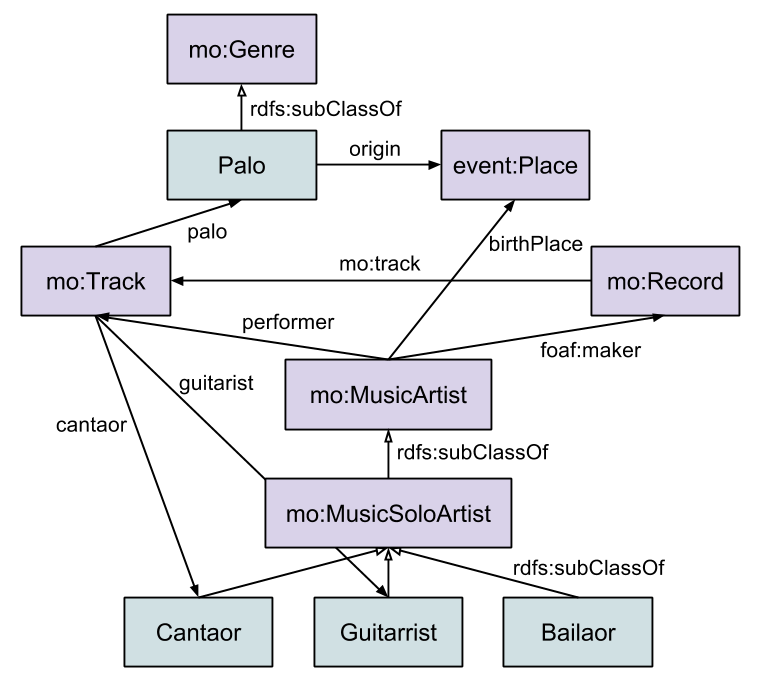
\includegraphics[width=0.40\textwidth]{ch08_musicology/pics/flabase_ontology2.png}
	\caption{Ontology schema \label{fig:ontology}}
\end{figure}
\fi



\subsection{Content Curation}\label{sec:kb_curation}

The first step towards building a domain-specific knowledge base is to gather all possible content from available data sources. This implies at least two problems, namely, the selection of sources, and the matching between entities from different sources. In what follows we enumerate the involved data sources and describe the methodology applied to entity resolution.

\subsubsection{Data Acquisition}\label{sec:datasoruces}

Our aim is to gather an important amount of information about musical entities, including textual descriptions and available metadata. A schema of the selected data sources is shown in Figure~\ref{fig:datasources}. We started by looking at Wikipedia\footnote{\url{http://www.wikipedia.org}}, the free and multilingual Internet encyclopedia. It is the Internet's largest and most popular general reference work. Each Wikipedia article may have a set of associated categories. Categories are intended to group together pages on similar subjects and are structured in a taxonomical way. To find Wikipedia articles related to flamenco music, we first looked for flamenco categories. The taxonomy of categories can be explored by querying DBpedia, a knowledge base with structured content extracted from Wikipedia. In particularly, we employed the SPARQL endpoint of the Spanish DBpedia\footnote{\url{http://es.dbpedia.org}}. We queried for categories related to the flamenco category in the taxonomy. At the end, we obtained 17 different categories (e.g., \textit{cantaores de flamenco, guitarristas de flamenco}).

\begin{figure}
	\centering
	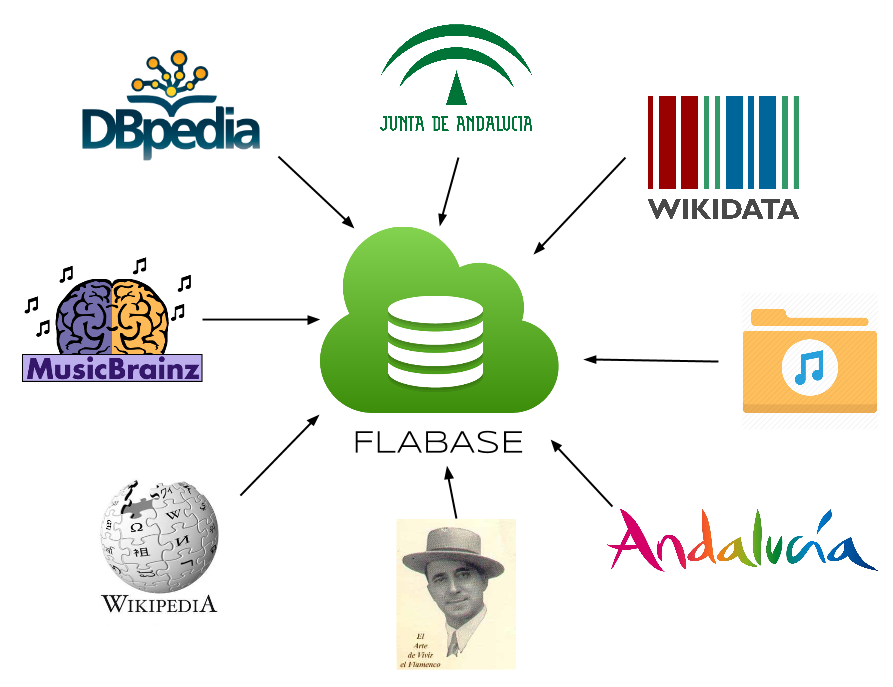
\includegraphics[width=0.45\textwidth]{ch08_musicology/pics/datasources.png}
	\caption{Selected data sources \label{fig:datasources}}
\end{figure}

%DBpedia resources are related to categories through the property dcterms:subject. Thus, b
By querying again DBpedia, we gathered all DBpedia resources related to one of these categories. We obtained a total number of 438 resources in Spanish, of which 281 were also in English. Each DBpedia resource is associated with a Wikipedia article. Text and HTML code were then extracted from Wikipedia articles in English and Spanish by using the WikiMedia API. 
%From DBpedia, we also gathered some biographical structured information of each resource, when it was available. 
Next, we classified the extracted articles according to the ontology schema defined in our knowledge base (Section~\ref{sec:ontology}). For this purpose, we exploited classification information provided by DBpedia (DBpedia ontology and Wikipedia categories). At the end, from all gathered resources, we only kept those related to artists and \textit{palos}, totalling  291 artists and 56 \textit{palos}.

However, the amount of information present in Wikipedia related to flamenco music is somewhat scarce. Therefore, we decided to expand our knowledge base with information from two different websites. First, \textit{Andalucia.org}, the touristic web from the Andalusia Government\footnote{\url{http://andalucia.org}}. It contains 422 artist biographies in English and Spanish, and the description of 76 \textit{palos} also in both languages. Second, a website called \textit{El arte de vivir el flamenco}\footnote{\url{http://www.elartedevivirelflamenco.com/}}, which includes 749 artist biographies among \textit{cantaores}, \textit{bailaores} and guitarists. Both webs were crawled and their content stored in our knowledge base. %As it is explained in Section~\ref{sec:entity_resolution}, artists from the three datasources were mapped, obtaining a final set of 1,176 different artists.

MusicBrainz is one of the biggest and more reliable open music databases, which provides an unambiguous form of music identification. Therefore, we turned to it in order to fill our knowledge base with information about flamenco album releases and recordings. Artists present in FlaBase were intended to be mapped with MusicBrainz artists. For every match, all content related to releases and recordings was gathered. After doing so, we obtained a total number of 814 releases and 9,942 recordings. 
%AcousticBrainz\footnote{\url{http://acousticbrainz.org}} is a project that aims to crowd source acoustic information for all music tracks identified in MusicBrainz. We queried the AcousticBrainz API for the acoustic descriptors of MusicBrainz recordings. We found acoustic information of 620 of the stored recordings.%, and kept it in our knowledge base.

The information gathered from MusicBrainz is a little part of the actual flamenco discography. Therefore, to complement it we used a flamenco recordings database gathered by Rafael Infante and available at CICA website\footnote{\url{http://flun.cica.es/index.php/grabaciones}} (Computing and Scientific Center of Andalusia). This database has information about releases from the early time of recordings until present time, counting 2,099 releases and 4,136 songs. For every song entry, a \textit{cantaor} name is provided, and most of the times also guitarist and \textit{palo}, which is a very valuable information to define flamenco recordings.

Finally, we supplied our knowledge base with information related to Andalusian towns and provinces. We gathered this information from the official database SIMA\footnote{\url{http://www.juntadeandalucia.es/institutodeestadisticaycartografia/sima}} (Multi-territorial System of Information of Andalusia).%, of the Official Institute of Statistics and Cartography of Andalusia. 


\subsubsection{Entity Resolution}\label{sec:entity_resolution}

Entity Resolution (ER) is the problem of extracting, matching and resolving entity mentions in structured and unstructured data \cite{Getoor2012}. There are several approaches to tackle the ER problem. For the scope of this research, we selected a pair-wise classification approach based on string similarity between entity labels.

The first issue after gathering the data is to decide whether two entities from different sources are referring to the same one. Therefore, given two sets of entities $A$ and $B$, the objective is to define an injective and non-surjective mapping function $f$ between $A$ and $B$ that decides whether an entity $a \in A$ is the same as an entity $b \in B$. To do that, a string similarity metric $sim(a,b)$ based on the Ratcliff-Obershelp algorithm \cite{Ratcliff1988} has been defined. It measures the similarity between two entity labels and outputs a value between 0 and 1. We consider that $a$ and $b$ are the same entity if their similarity is bigger than a parameter $\theta$. If there are two entities $b, c \in B$ that satisfy that $sim(a,b) \geq \theta$ and $sim(a,c) \geq \theta$, we consider only the mapping with the highest score. To determine the value of $\theta$, we tested the method with several $\theta$ values over an annotated dataset of entity pairs. To create this dataset, the 291 artists gathered from Wikipedia were manually mapped to the 422 artists gathered from Andalucia.org, obtaining a total amount of 120 pair matches. As it is shown in Figure~\ref{fig:fmeasure} the best F-measure (0,97) was obtained with $\theta=0.9$. Finally, we applied the described method with $\theta=0.9$ to all gathered entities from the three data sources. Thanks to the entity resolution process, we reduced the initial set of 1,462 artists and 132 \textit{palos} to a set of 1,174 artists and 76 \textit{palos}.

\begin{figure}
	\centering
	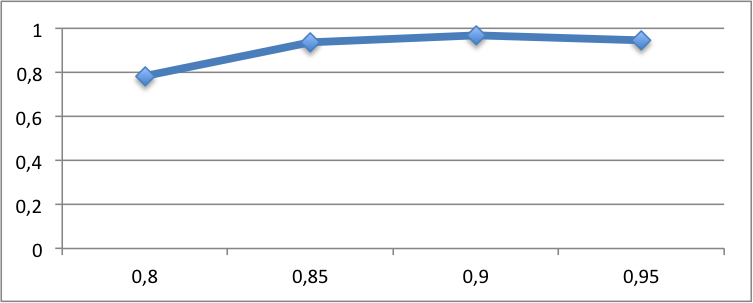
\includegraphics[width=0.40\textwidth]{ch08_musicology/pics/similarity_f.png}
	\caption{F-measure for different values of $\theta$ \label{fig:fmeasure}}
\end{figure}

Once we had our artist entities resolved, we began to gather their related discographic information. First, we tried to find out the MusicBrainz ID of the gathered artists. Depending on the information about the entity, two different process were applied. First, every Wikipedia page, and its equivalent DBpedia resource, has a correspondent entity defined in Wikidata. Wikidata is a free linked database which acts as a structured data storage of Wikipedia. There are several properties in Wikidata that may link Wikidata items with MusicBrainz items. Thus, the equivalent Wikidata resource of a Wikipedia artist page may have a link to its corresponding MusicBrainz artist ID. Therefore, we looked for these relations and mapped all possible entities. For those artists without a direct link to MusicBrainz, we queried the MusicBrainz API by using the artist labels, and then applied our entity resolution method to the obtained results.

Finally, to integrate the discography database of CICA into our knowledge base, we applied the entity resolution method to the fields \textit{cantaor}, guitarist and \textit{palo} of each recording entry in the database. From the set of 202 \textit{cantaores} and 157 guitarists names present in the recording entries, a total number of 78 \textit{cantaores} and 44 guitarists were mapped to our knowledge base. The number of mapped artists was low due to differences between the way of labeling an artist. An artist name may be written using one or two surnames, or using a nickname. In the case of \textit{palos}, there were 162 different \textit{palos} in the database, 54 of which were mapped with the 76 of our knowledge base. These 54 \textit{palos} correspond to an 80\% of \textit{palo} assignments present in the recording entries.


\subsection{Knowledge Extraction}\label{sec:kb_extraction}

Once the process of data acquisition is finished, the knowledge base is ready for use. However, there is an important amount of knowledge present in the data that has not been fully exploited. Texts gathered contain a huge epistemic potential that remains implicit. Consequently, to enhance the amount of structured data in FlaBase, a process of knowledge extraction has been carried out. This implicit knowledge may vary from biographical data, such as place and date of birth, to more complex semantic relations involving different entities. Three tasks play a key role in the process of knowledge extraction from non-structured text: named entity recognition (NER), named entity disambiguation (NED), and relation extraction (RE) \cite{Usbeck2014}. In this research, we focus on the two first tasks. In what follows, a system for entity recognition and disambiguation is described and evaluated. Lastly, an information extraction process is applied to populate the knowledge base.

\subsubsection{Named entity recognition and disambiguation}\label{sec:entity_linking}

To extract implicit knowledge from a text, the first step is to semantically annotate it by identifying entity mentions. Named entity recognition is a task that seeks and classify words in text into pre-defined categories (e.g., person, organization, or place). Named entity disambiguation, also called entity linking, aims to determine what is actually a named entity present in a text. It generally does so by identifying it in a knowledge base of reference. NED can be addressed directly from the text, or applied to the output of a NER system. We propose a method that employs a combination of both approaches, depending on the category of the entity. For NER, we used the Stanford NER system \cite{Finkel2005}, implemented in the library Stanford Core NLP\footnote{\url{http://nlp.stanford.edu/software/corenlp.shtml}} and trained on Spanish texts. For NED we tried two different approaches. First, we looked for exact string matches between FlaBase entity labels and word n-grams extracted from the text. Second, we searched for exact string matches between FlaBase entity labels and the output of the NER system. In fact, we tried several combinations of both approaches until we obtained the most satisfactory one.

%We selected all biography texts in Spanish from artists present in our knowledge base. 
For the scope of this research, we focused on Spanish texts, as flamenco texts are mostly written in Spanish. Although there are many entity linking tools available, we decided to develop ours because state-of-the-art systems (e.g., Tag-me or Babelfy) are well-tuned for English texts, but do not perform well on Spanish texts, and even less with music texts of a specific domain. In addition, we wanted to have a system able to map entities to our knowledge base. Therefore, we developed a system able to detect and disambiguate three categories of entities: person, \textit{palo} and location. Three different approaches were defined by combining NER and NED in different ways according to the category. First, directly applying NED to text. Second, disambiguating location and person entities from the NER output, and \textit{palo} directly from text. Third, only disambiguating location entities from the NER output, and location and \textit{palo} directly from text.

To determine which approach performs better, three artist biographies coming from three different data sources were manually annotated, having a total number of 49 annotated entities. We followed an evaluation methodology similar to the one used in KBP2014 Entity Linking Task\footnote{\url{http://nlp.cs.rpi.edu/kbp/2014/}}. Results on the different approaches are shown in Table~\ref{tbl:res1}. We observe that applying NER to entities of the person category before NED worsens performance significantly, as recall suddenly decrease by half. After manually analysing false negatives, we observed that this is caused because many artist names have definite articles between name and surname (e.g., \textit{de, del}), and this is not recognized by the NER system. In addition, many artists have a nickname that is not interpreted as a person entity by the NER system. The best approach is the third (NED + NER to LOC), which is slightly better than the first (only NED) in terms of precision. This is due to the fact that many artists have a town name as a surname or as part of his nickname. Therefore, applying NED directly to text is misclassifying person entities as location entities. Thus, by adding a previous step of NER to location entities we have increased overall performance, as it can be seen on the F-measure values.

\begin{table}
	\centering
%\begin{adjustbox}{max width=8cm}
	  \begin{tabular}{ | l | c | c | c | }
    \hline
    Approach & Precision & Recall & F-measure \\ \hline
    \hline
    1) NED & 0.829 & \textbf{0.694} & 0.756 \\ 
    2) NED + NER to PERS \& LOC & 0.739 & 0.347 & 0.472 \\
    3) NED + NER to LOC & \textbf{0.892} & 0.674 & \textbf{0.767} \\
    \hline
  \end{tabular}
%  \end{adjustbox}
	\caption{Precision, Recall and F-measure of NER+NED}
	
	\label{tbl:res1}
\end{table}

\subsubsection{Knowledge base population}\label{sec:ie}

Biographical texts coming from different data sources have been stored in FlaBase. These texts are full of relevant information about FlaBase entities, but in an unstructured way. Thus, a process of information extraction is necessary to transform the unstructured information into structured knowledge. For the scope of this research, we focused on extracting two specific data: birth year and birth place, as they can be very relevant for anthropologic studies. We observed that this information is often in the very first sentences of the artist biographies, and always near the word \textit{naci\'{o}} (Spanish translation of ``was born"). Therefore, to extract this information, we looked for this word in the first 250 characters of every biographical text. If it is found, we apply our entity linking method to this piece of text. If a location entity is found near the word "naci\'{o}", we assume that this entity is the place of birth of the biography subject. In addition, by using regular expressions, we look for the presence of a year expression in the neighborhood. If it is found, we assume it as the year of birth. If more than one year is found, we select the one with the smaller value. 

To evaluate our approach, we tested the extraction of birth places in all texts coming from the web Andalucia.org (442 artists). We chose this subset because Andalucia.org also provides specific information about artist origin that had been previously crawled and stored in FlaBase. However, we observed that in many occasions the artist origin provided by the data source was wrong. Therefore, we decided to manually annotate the province of precedence of these 442 artists for building ground truth data. After the application of the extraction process on the annotated test set, we obtained a precision value of 0,922 and a recall of 0,648. Therefore, we can state that our method is extracting biographic information with very high precision and quite reasonable recall. 
%In addition, the information extracted by our system is indeed more accurate than the actual information provided by the data source. 
We finally applied the extraction process to all artist entities with biographical texts coming from any of the two flamenco crawled websites. Thus, from a total number of 1,123 artists coming from these data sources (95\% of the artists in the knowledge base), 743 birth places and 879 birth years were extracted. 


\section{Exploring Music Digital Libraries}




\section{Diachronic Study of Music Criticism}\label{sec:evolution}

We carried out a study of the evolution of music criticism from two different temporal standpoints. Specifically, we consider when the review was written and, in addition, when the album was first published. Since we have sentiment information available for each review, we first computed an average sentiment score for each year of review publication (between 2000 and 2014). In this way, we may detect any significant fluctuation in the evolution of affective language during the 21st century. Then, we also calculated the average sentiment for each review by year of album publication. This information is obtained from MB and complemented with the average of the Amazon rating scores.

In what follows, we show visualizations for sentiment scores and correlation with ratings given by Amazon users, according to these two different temporal dimensions. Although arriving to musicological conclusions is out of the scope of this paper, we provide \textit{food for thought} and present the readers with hypotheses that may explain some of the facts revealed by these data-driven trends.

%We carried out a study of the evolution of music criticism from two different temporal standpoints. Specifically, we consider when the review was written and, in addition, when the release was first published. On the one hand, we computed the average sentiment polarity score according to the year of publication of the reviews. This approach let us observe how the polarity associated to language used for describing music has evolved during the 21st century. On the other hand, we calculated average sentiment polarity by year of release of the reviewed albums. Thanks to the enrichment applied to the dataset, we were able to gather this information from MusicBrainz. In both cases, we also computed the average of the Amazon rating scores provided within the reviews.
%In what follows, we show some plots of the computed sentiment and rating scores, according to the two different perspectives. Although arrive to musicological conclusions is out of the scope of this paper, we suggest some possible hypothesis that may explain the causes of the observations made in the data.

\begin{figure*}[ht!]
    \centering
    \begin{subfigure}{.3\textwidth}
        \centering
        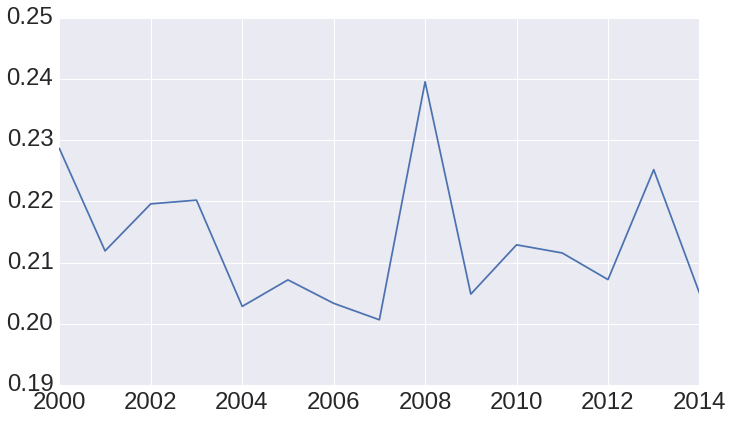
\includegraphics[width=.9\linewidth]{ch08_musicology/pics/all_average.png}
        \caption{Sentiment}
        \label{fig:avgSentReview}
    \end{subfigure}
    \begin{subfigure}{.3\textwidth}
        \centering
        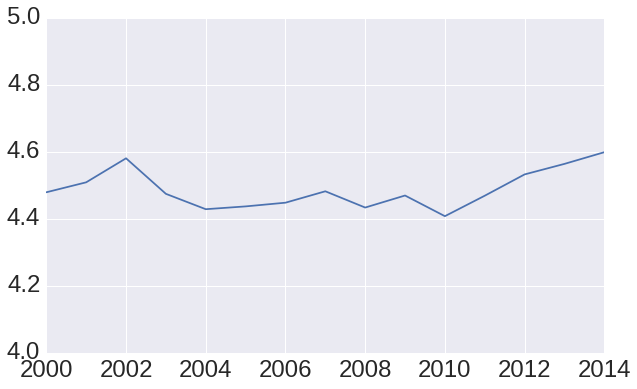
\includegraphics[width=.9\linewidth]{ch08_musicology/pics/avg_score.png}
        \caption{Rating}
        \label{fig:avgRatingReview}
    \end{subfigure}
    %\begin{subfigure}{.3\textwidth}
    %    \centering
    %    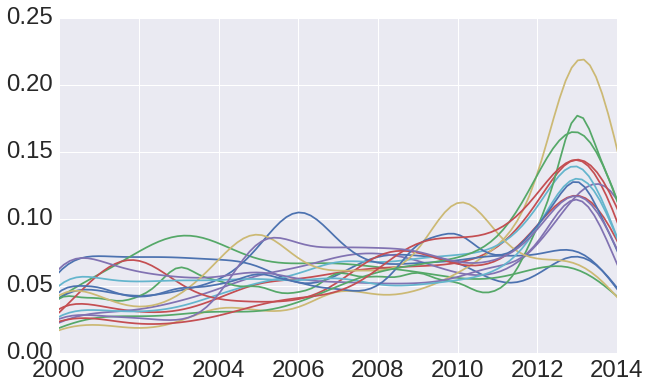
\includegraphics[width=.9\columnwidth]{ch08_musicology/pics/kde.png}
    %    \caption{Kernel density estimation}
    %    \label{fig:kde}
    %\end{subfigure}
    %\begin{subfigure}{.3\textwidth}
    %    \centering
    %    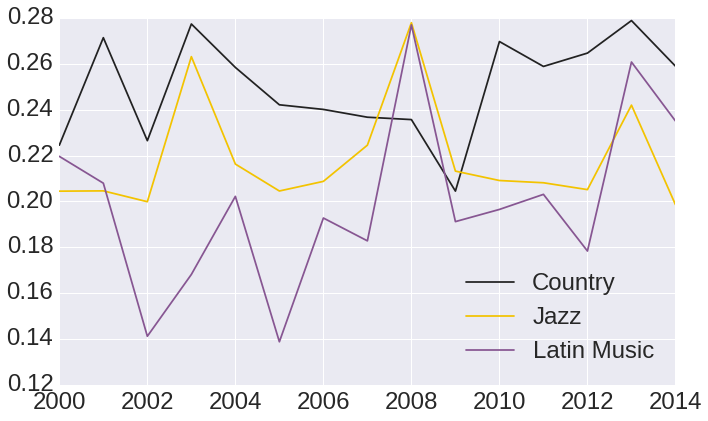
\includegraphics[width=.9\linewidth]{ch08_musicology/pics/genres_average.png}
    %    \caption{Sentiment by genre}
    %    \label{fig:avgSentReviewGenres}
    %\end{subfigure}
    %\begin{subfigure}{.3\textwidth}
    %    \centering
    %    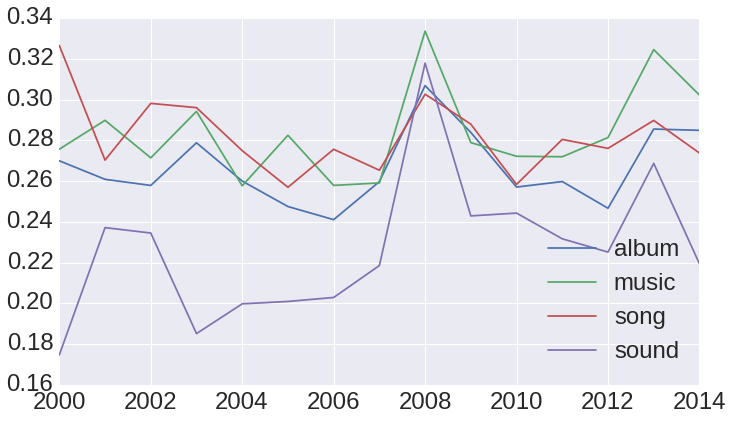
\includegraphics[width=.9\linewidth]{ch08_musicology/pics/main_aspects.png}
    %    \caption{Sentiment by aspect}
    %    \label{fig:avgSentReviewAspects}
    %\end{subfigure}
    \begin{subfigure}{.3\textwidth}
        \centering
        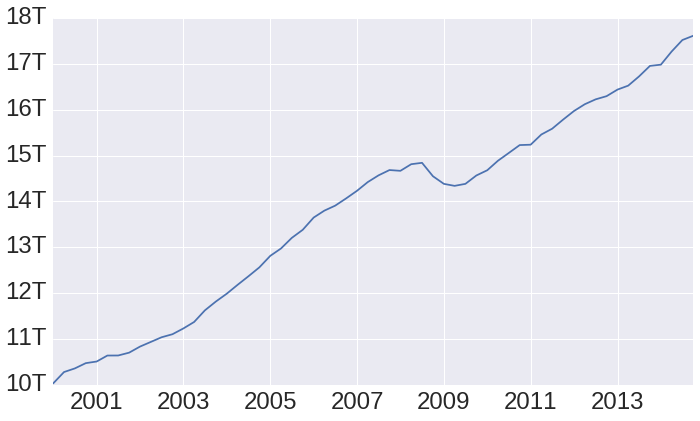
\includegraphics[width=.8\linewidth]{ch08_musicology/pics/gdp2.png}
        \caption{USA GDP trend}
        \label{fig:gdp}
    \end{subfigure}
 
   \begin{subfigure}{.3\textwidth}
        \centering
        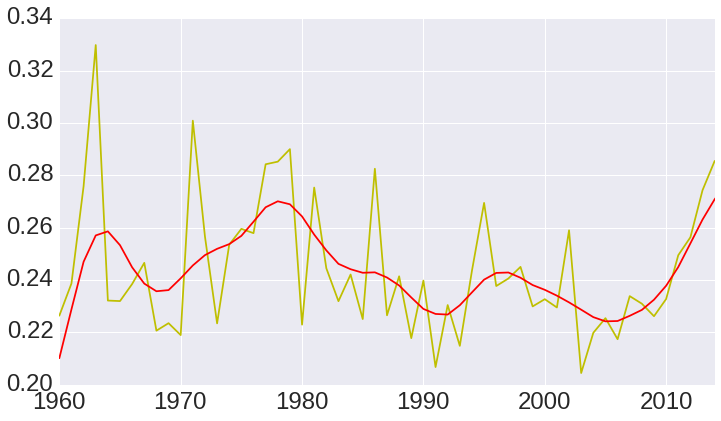
\includegraphics[width=.9\textwidth]{ch08_musicology/pics/sentiment_release_trend.png}
        \caption{Sentiment}
        \label{fig:avgSentimentRelease}
    \end{subfigure}
    \begin{subfigure}{.3\textwidth}
        \centering
        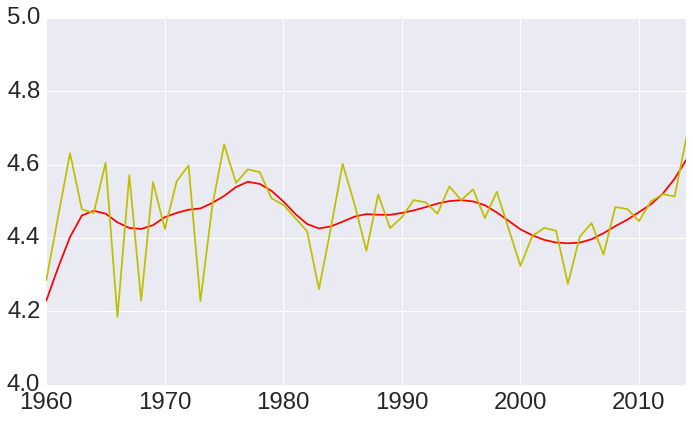
\includegraphics[width=.9\textwidth]{ch08_musicology/pics/rating_release_trend.png}
        \caption{Rating}
        \label{fig:avgRatingRelease}
    \end{subfigure}
    \begin{subfigure}{.3\textwidth}
        \centering
        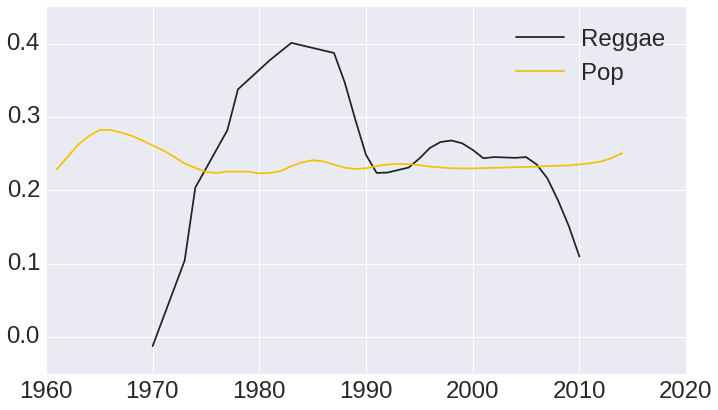
\includegraphics[width=.9\columnwidth]{ch08_musicology/pics/genres_release_trend.png}
        \caption{Sentiment by genre}
        \label{fig:avgSentimentGenresRelease}
    \end{subfigure}
    \caption{Sentiment and rating averages by review publication year (a and b); GDP trend in USA from 2000 to 2014 (c), and sentiment and rating averages by album publication year (d, e and f)}
    %\caption{Sentiment and rating averages by review publication year (a, b d and e); Kernel density estimation of the distribution of reviews by year (c); GDP trend in USA from 2000 to 2014 (f), and sentiment and rating averages by album publication year (g, h and i)}
\end{figure*}

\subsection{Evolution by Review Publication Year}

We applied sentiment and rating average calculations to the whole MARD dataset, grouping album reviews by year of publication of the review. Figure \ref{fig:avgSentReview} shows the average of the sentiment scores associated to every aspect identified by the sentiment analysis framework in all the reviews published in a specific year, whilst Figure~\ref{fig:avgRatingReview} shows average review ratings per year. At first sight, we do not observe any correlation between the trends illustrated in the figures. However, the sentiment curve (Figure~\ref{fig:avgSentReview}) shows a remarkable peak in 2008, a slightly lower one in 2013, and a low between 2003 and 2007, and also between 2009 and 2012. %Figure~\ref{fig:kde} shows the kernel density estimation of the distribution of reviews by year of the 16 genres. The shape of these curves suggest that the 2008 peak in the sentiment score is not related to the number of reviews published that year. The peak persists if we construct the graphs with the average sentiment associated with the most repeated aspects in text (Figure \ref{fig:avgSentReviewAspects}). 
It is not trivial to give a proper explanation of this variations on the average sentiment. We speculate that these curve fluctuations may suggest some influence of economical or geopolitical circumstances in the language used in the reviews, such as the 2008 election of Barack Obama as president of the US. As stated by the political scientist Dominique Mo\"{i}si in \cite{Moisi2010}:

\begin{displayquote}\small{
In November 2008, at least for a time, hope prevailed over fear. The wall of racial prejudice fell as surely as the wall of oppression had fallen in Berlin twenty years earlier [...] Yet the emotional dimension of this election and the sense of pride it created in many Americans must not be underestimated.}
\end{displayquote}

Another factor that might be related to the positiveness in use of language is the economical situation. After several years of continuous economic growth, in 2007 a global economic crisis started\footnote{\url{https://research.stlouisfed.org}}, whose consequences were visible in the society after 2008 (see Figure~\ref{fig:gdp}). In any case, further study of the different implied variables is necessary to reinforce any of these hypotheses.

%Assuming that a vast majority of reviewers are North American (we do not have this information available), as the dataset was originally gathered from Amazon US, these trends may be explained with the 2008 election of president Barack Obama as president of the US. As stated by Dominique Mo\"{i}si in \cite{Moisi2010}:
%We assume that a vast majority of reviewers should be from the United States, as the dataset was originally gathered from the American version of the Amazon website.  
%Starting from this assumption, an important event happened in 2008 which affected not only United States citizens but the entire world, the election of Barak Obama as the President of the United Sates. As stated by Dominique Moïsi in \cite{Moisi2010}:

%If we calculate the sentiment evolution curve for the different genres (see Figure~\ref{fig:avgSentReviewGenres}), we observe that 2008 constitutes an all-time-high for almost all genres. It is remarkable that genres traditionally related to Black and Hispanic communities such as Jazz and Latin Music experience such an increase, whilst other genres such as Country do not
. 
%Another factor that might be related to the positiveness in use of language is the economical situation. After several years of continuous economic growth, in 2007 a global economic crisis started, originated by the subprime mortgage crisis, whose consequences were more visible in the society from 2009 to 2013\footnote{\url{https://research.stlouisfed.org}}, as shown in Figure~\ref{fig:gdp}. %Following this hypothesis, the abrupt decrease of positiveness right after 2008 and its recovery by 2013 might be related to this. 
%In any case, further study of the different implied variables is necessary to reinforce any of these hypotheses.
    

%\begin{figure}
%    \centering
%    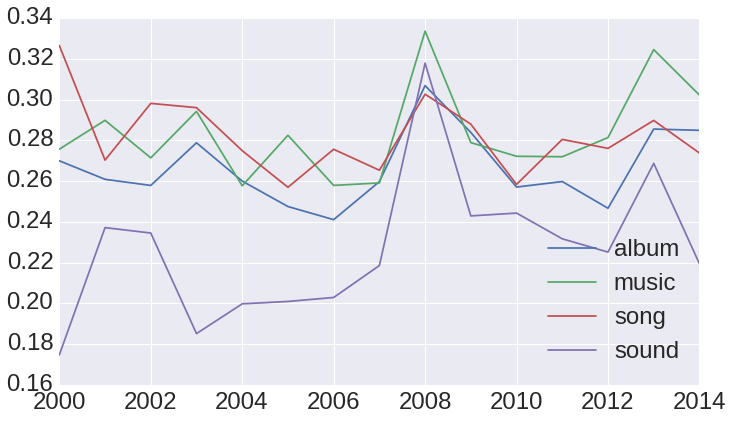
\includegraphics[width=.6\columnwidth]{ch08_musicology/pics/main_aspects.png}
%    \caption{Average sentiment of main aspects across genres by review year}
%    \label{fig:avgSentimentGenresReview}
%\end{figure}


\subsection{Evolution by Album Publication Year}

In this case, we study the evolution of the polarity of language by grouping reviews according to the album publication date. This date was gathered from MB, meaning that this study is conducted on the ~42,1\% of the MARD that was successfully mapped. We compared again the evolution of the average sentiment polarity (Figure~\ref{fig:avgSentimentRelease}) with the evolution of the average rating (Figure~\ref{fig:avgRatingRelease}). Contrary to the results observed by review publication year, here we observe a strong correlation between ratings and sentiment polarity. To corroborate that, we computed first a smoothed version of the average graphs, by applying 1-D convolution (see line in red in Figures~\ref{fig:avgSentimentRelease} and \ref{fig:avgRatingRelease}). Then we computed Pearson's correlation between smoothed curves, obtaining a correlation $r = 0.75$, and a p-value $p \ll 0.001$. This means that in fact there is a strong correlation between the polarity identified by the sentiment analysis framework in the review texts, and the rating scores provided by the users. This correlation reinforces the conclusions that may be drawn from the sentiment analysis data. %, and reinforces the idea of averaging local sentiment scores as a measure of polarity in a review. %These sentiment scores might be used as an important feature for a rating prediction task.

To further dig into the utility of this polarity measure for studying genre evolution, we also computed the smoothed curve of the average sentiment by genre, and illustrate it with two idiosyncratic genres, namely \textit{Pop} and \textit{Reggae} (see  Figure~\ref{fig:avgSentimentGenresRelease}). We observe in the case of \textit{Reggae} that there is a time period where reviews have a substantial use of a more positive language between the second half of the 70s and the first half of the 80s, an epoch which is often called the golden age of \textit{Reggae} \cite{alleyne2012encyclopedia}. This might be related to the publication of Bob Marley albums, one of the most influential artists in this genre, and the worldwide spread popularity of reggae music. In the case of \textit{Pop}, we observe a more constant sentiment average. However, in the 60s and the beginning of 70s there are higher values, probably consequence by the release of albums by The Beatles. These results show that the use of sentiment analysis on music reviews over certain timelines may be useful to study genre evolution and identify influential events.


\section{Conclusions}

Our diachronic study of the sentiment polarity expressed in customer reviews explores two interesting ideas. First, the analysis of reviews classified by year of review publication suggests that geopolitical events or macro-economical circumstances may influence the way people speak about music. Second, an analysis of the reviews classified by year of album publication is presented. The results show how sentiment analysis can be very useful to study the evolution of music genres. The correlation observed between average rating and sentiment scores suggest the suitability of the proposed sentiment-based approach to predict user satisfaction with musical products. Moreover, according to the observed trend curves, we can state that we are now in one of the best periods of the recent history of music.  %The observed trend curves suggest that we are in one of the best periods of the recent history of music.
Further work is necessary to elaborate on these hypotheses. In addition, the combination of audio and textual features is still an open problem, not only for classification but also for the study of the evolution of music. We expect the released dataset will be explored in multiple ways for the development of multimodal research approaches in MIR.
%, especially considering the availability of massive repositories of musical data.
In conclusion, the main contribution of this work is a demonstration of the utility of applying systematic linguistic processing on texts about music. Furthermore, we foresee our method to be of interest for musicologists, sociologists and humanities researchers in general.
%To conclude, and far from arriving to musicological conclusions, the main contribution of this paper is the demonstration of the utility of applying systematic linguistic processing on texts about music. Furthermore, we foresee our method to be of interest for musicologists, sociologists and humanities researchers in general.